\documentclass[conference]{IEEEtran}

\usepackage{cite}
\usepackage{amsmath,amssymb,amsfonts}
\usepackage{graphicx}
\usepackage{textcomp}
\usepackage{xcolor}
\usepackage{booktabs}
\usepackage{algorithmic}
\usepackage{algorithm}
\usepackage{hyperref}
\usepackage{tikz}
\usetikzlibrary{shapes.geometric, arrows.meta, positioning, fit, calc}

\hypersetup{
    colorlinks=true,
    linkcolor=black,
    citecolor=black,
    urlcolor=blue!70!black,
}

\begin{document}

\title{SignAction: A Modular Pipeline for Translating Text and Speech into Indian Sign Language Gestures}

\author{
\makebox[\textwidth][c]{%
\begin{tabular}{@{}c@{\hspace{1.1cm}}c@{\hspace{1.1cm}}c@{}}
\begin{minipage}[t]{0.29\textwidth}
\centering
{\normalsize $1^{\mathrm{st}}$ Roma Kudale}\\
{\normalsize\textit{Dept of AI\&DS}}\\
\textit{CMR Institute of Technology}\\
Banagalore. India\\
\href{mailto:roma.k@cmrit.ac.in}{roma.k@cmrit.ac.in}
\end{minipage}
&
\begin{minipage}[t]{0.29\textwidth}
\centering
{\normalsize $2^{\mathrm{nd}}$ C Vishwak Sena}\\
{\normalsize\textit{Dept of CS\&DS}}\\
\textit{CMR Institute of Technology}\\
Banagalore. India\\
\href{mailto:chilukurvishwak21@gmail.com}{chilukurvishwak21@gmail.com}
\end{minipage}
&
\begin{minipage}[t]{0.29\textwidth}
\centering
{\normalsize $3^{\mathrm{rd}}$ Ananya U}\\
{\normalsize\textit{Dept of AI\&DS}}\\
\textit{CMR Institute of Technology}\\
Banagalore. India\\
\href{mailto:uananya324@gmail.com}{uananya324@gmail.com}
\end{minipage}
\\
\noalign{\vskip 1.2em}
\begin{minipage}[t]{0.29\textwidth}
\centering
{\normalsize $4^{\mathrm{th}}$ Ashirwad}\\
{\normalsize\textit{Dept of AI\&DS}}\\
\textit{CMR Institute of Technology}\\
Banagalore. India\\
\href{mailto:ashirwads813@gmail.com}{ashirwads813@gmail.com}
\end{minipage}
&
\begin{minipage}[t]{0.29\textwidth}
\centering
{\normalsize $5^{\mathrm{th}}$ Aditya Mule}\\
{\normalsize\textit{Dept of AI\&DS}}\\
\textit{CMR Institute of Technology}\\
Banagalore. India\\
\href{mailto:adityamule79@gmail.com}{adityamule79@gmail.com}
\end{minipage}
& {}
\end{tabular}%
}
}

\maketitle

% =============================================================
% ABSTRACT
% =============================================================
\begin{abstract}
A 2016 annual-report estimate from the National Association of the Deaf put India's deaf population at 18 million, although national estimates vary considerably \cite{sharma2025}. Continuous English--Indian Sign Language (ISL) resources have grown, but annotated parallel data remain limited, while dictionary-only systems cannot represent how signs connect in a sentence. This paper presents SignAction, a system that takes English text or recorded speech and produces animated ISL gesture sequences. A rule-based NLP module turns input text into gloss tokens. A file-based resolver checks those tokens against a folder of pre-recorded sign files. We gathered these sign files from free animated ISL video datasets online. If nothing matches, a synthesizer draws a stick-figure animation using sign parameters manually derived by the authors from ISLRTC dictionary videos. A FastAPI server exposes the pipeline over REST, and a Next.js frontend handles text input, audio recording, and gesture playback. On a test set of 320 English sentences, the glosser got about 93\% token-level accuracy. The time from text to first gesture frame was around 100\,ms. The whole thing runs on one CPU core with no GPU.
\end{abstract}

\begin{IEEEkeywords}
Indian Sign Language, sign language translation, speech-to-text, natural language processing, accessibility, gesture synthesis
\end{IEEEkeywords}

% =============================================================
% 1. INTRODUCTION
% =============================================================
\section{Introduction}
\label{sec:intro}

Linguistic research established signed languages as structured natural languages \cite{stokoe1960, klima1979}, yet sign-language recognition, generation, and translation remain comparatively underrepresented in language technology research \cite{bragg2019}. The WHO estimated in 2021 that 430 million people had disabling hearing loss and projected that more than 700 million would have disabling hearing loss by 2050 \cite{who2021}. For many deaf people, sign language is a primary means of learning, work, and social communication \cite{bragg2019}.

Building a translation system between spoken and signed language is interdisciplinary: it combines linguistics, computer vision, human--computer interaction, and Deaf-community considerations \cite{bragg2019}. Large data-driven systems require aligned and annotated visual-language corpora \cite{camgoz2020}, and ISL remains resource-limited compared with several better-studied sign languages \cite{joshi2024isign}. The third edition of the ISLRTC dictionary contained 10{,}000 terms \cite{islrtc2021}; INCLUDE and CISLR provide isolated or word-level sign videos \cite{sridhar2020, joshi2022cislr}, while ISLTranslate and iSign introduced continuous ISL--English pairs and broader processing benchmarks \cite{joshi2023isltranslate, joshi2024isign}. These resources are important, but models trained for ASL or German Sign Language cannot be transferred to ISL without adaptation to its linguistic and spatial conventions \cite{joshi2024isign}.

We built SignAction to work without training on a large parallel corpus. The pipeline has three steps. A rule-based NLP module turns English text into gloss tokens. Those tokens are matched against a folder of sign files (GIFs, MP4s, images). If a token has no match, a stick-figure animation is drawn on the fly using hand-position and movement parameters that we manually derived from ISLRTC dictionary videos.

This paper makes four concrete contributions:
\begin{itemize}
    \item A pipeline with three independent stages (NLP, asset lookup, rendering) so that any stage can be swapped without touching the others.
    \item A fallback renderer that draws a stick-figure animation for any unknown word, so the output is never blank.
    \item A fingerspelling fallback that splits unknown alphabetic words into letters and looks up each letter separately.
    \item A web application supporting text, speech, and audio file upload that runs on a regular cloud VM with no GPU.
\end{itemize}

Section~\ref{sec:related} covers related work. Section~\ref{sec:arch} describes the architecture. Section~\ref{sec:method} walks through each pipeline stage. Section~\ref{sec:results} presents results and discusses shortcomings. Section~\ref{sec:conclude} wraps up.

% =============================================================
% 2. RELATED WORK
% =============================================================
\section{Related Work}
\label{sec:related}

\subsection{Sign Language Recognition}

Stokoe \cite{stokoe1960} published the first modern linguistic analysis of a signed language and represented ASL signs through location, handshape, and movement. These parameters remain influential in computational descriptions of signs \cite{cooper2012}. Klima and Bellugi \cite{klima1979} provided a broader linguistic account of ASL and demonstrated systematic structure beyond isolated gestures.

On the machine learning side, Camgoz et al. \cite{camgoz2020} trained a transformer model on RWTH-PHOENIX-Weather, a German Sign Language dataset of weather forecast broadcasts. It works in that narrow domain, but it needs aligned video--text pairs and substantial training data.

For ISL, Sridhar et al. \cite{sridhar2020} introduced INCLUDE, a dataset for isolated-sign recognition, and Joshi et al. \cite{joshi2022cislr} introduced CISLR for word-level recognition. ISLTranslate later supplied approximately 31{,}000 continuous ISL--English sentence or phrase pairs \cite{joshi2023isltranslate}, while iSign expanded the available data and benchmarked several recognition, translation, and sign-production tasks \cite{joshi2024isign}. ISLRTC also publishes a dictionary that maps ISL signs to English terms \cite{islrtc2021}, and that is the resource our asset lookup is built around.

Cooper et al. \cite{cooper2012} describe manual sub-units for handshape, location, hand arrangement, motion, and orientation, while also noting non-manual features. Many of these sub-units occur in parallel. A gloss sequence therefore cannot encode every visual distinction. We keep that in mind by playing gestures one after another rather than merging them into one image.

\subsection{Glossing as an Intermediate Representation}

Glossing---representing signs with spoken-language labels---has long been used in sign-language research \cite{klima1979}. Neidle et al. \cite{neidle2001} built SignStream, a tool for detailed annotation and analysis of ASL video. As an implementation convention, SignAction represents glosses as uppercase tokens and uses underscores to join multiword lexical items.

Huang et al. \cite{huang2018} showed that continuous sign sequences can be recognised without first segmenting a video into isolated signs. In SignAction, the gloss sequence is therefore used as a practical token-level interface, not as a complete representation of sign timing or simultaneous features.

The biggest weakness of gloss-based approaches is ambiguity. The word ``bank'' means a financial institution in one sentence and a riverbank in another, and a rule-based glosser cannot tell which is which from context alone. We handle a few fixed cases through alias and phrase tables, but general word-sense disambiguation is not in scope here.

\subsection{Gesture Synthesis}

Avatar-based sign synthesis has been around for a while, and Rastgoo et al. \cite{rastgoo2021} survey the progression from rule-based avatars to deep sign-production models. VSigns \cite{papadogiorgaki2004} was an early web tool that converted text to SignWriting and produced VRML avatar animations. More recent neural systems include Text2Sign, which combines neural translation, motion graphs, and video generation \cite{stoll2020}, and Progressive Transformers, which learn continuous 3D skeletal pose sequences from paired spoken-language and sign-language data \cite{saunders2020}. Such methods are promising, but they depend on parallel training data that SignAction is designed not to require.

We went a simpler route: stick figures. For the AI fallback signs, we manually viewed the corresponding ISLRTC dictionary videos and encoded simplified handshape, body-location, and movement parameters. The renderer reads these author-created definitions and draws 320$\times$360-pixel animated GIFs of a skeleton doing each sign. We give up realism to get coverage. Any token can produce an animation, not just ones that have pre-recorded video.

\subsection{Offline Speech Recognition}

Speech recognition in SignAction has to work offline. Vosk \cite{vosk2021} is a lightweight STT engine based on Kaldi \cite{povey2011}. Its 40\,MB small English model is listed at 9.85\% WER on LibriSpeech test-clean and 10.38\% on TED-LIUM \cite{vosk2021}. These benchmark results do not guarantee general dictation accuracy, but the model is adequate when the glosser mainly needs content words. Whisper \cite{radford2023} is available as an optional backend for cases where accuracy matters more than model size.

% =============================================================
% 3. SYSTEM ARCHITECTURE
% =============================================================
\section{System Architecture}
\label{sec:arch}

SignAction is split into three parts: a Next.js frontend, a FastAPI backend, and a Python library called \texttt{signaction}. The frontend and backend talk over REST. The backend calls the library for all translation work. Fig.~\ref{fig:arch} shows how data moves through the system.

\begin{figure}[t]
\centering
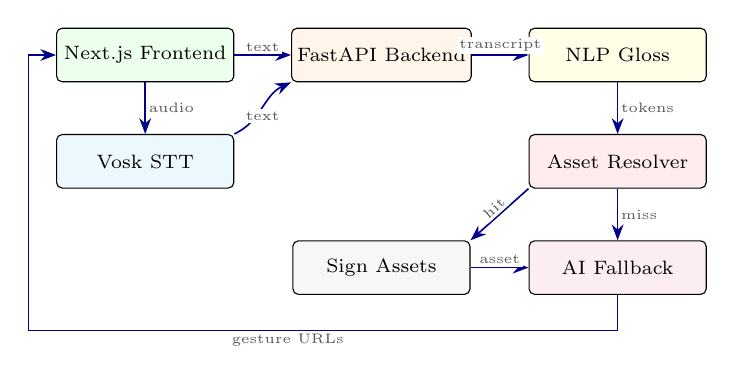
\begin{tikzpicture}[
    x=1cm,
    y=1cm,
    block/.style={rectangle, draw, fill=blue!6, minimum width=2.25cm,
                  minimum height=0.68cm, align=center, rounded corners=2pt,
                  inner sep=2pt, font=\scriptsize},
    arrow/.style={-{Stealth[length=2mm]}, semithick, color=blue!55!black},
    lbl/.style={font=\tiny, fill=white, inner sep=1pt,
                text=gray!70!black},
]
\node[block, fill=green!7]  (fe)   at (0,0)     {Next.js Frontend};
\node[block, fill=orange!8] (be)   at (3,0)     {FastAPI Backend};
\node[block, fill=yellow!10](nlp)  at (6,0)     {NLP Gloss};
\node[block, fill=cyan!8]   (stt)  at (0,-1.35) {Vosk STT};
\node[block, fill=red!7]    (map)  at (6,-1.35) {Asset Resolver};
\node[block, fill=gray!6]   (lib)  at (3,-2.70) {Sign Assets};
\node[block, fill=purple!7] (rend) at (6,-2.70) {AI Fallback};

\draw[arrow] (fe.east) -- node[above, lbl] {text} (be.west);
\draw[arrow] (be.east) -- node[above, lbl] {transcript} (nlp.west);
\draw[arrow] (fe.south) -- node[right, lbl] {audio} (stt.north);
\draw[arrow] (stt.north east) to[out=25, in=-155]
    node[pos=0.50, below, lbl] {text} (be.south west);
\draw[arrow] (nlp.south) -- node[right, lbl] {tokens} (map.north);
\draw[arrow] (map.south west) -- node[sloped, above, lbl] {hit}
    (lib.north east);
\draw[arrow] (map.south) -- node[right, lbl] {miss} (rend.north);
\draw[arrow] (lib.east) -- node[above, lbl] {asset} (rend.west);
\draw[arrow] (rend.south) -- ++(0,-0.45) -| node[pos=0.28, below, lbl]
    {gesture URLs} ([xshift=-0.35cm]fe.west) -- (fe.west);
\end{tikzpicture}
\caption{Data flow through SignAction. Text or audio enters the FastAPI backend, passes through NLP and asset resolution, and returns gesture URLs to the frontend.}
\label{fig:arch}
\end{figure}

\subsection{Frontend}

The client is a Next.js 14 app built with React 18 and Tailwind CSS. It has four views:

\begin{itemize}
    \item \textbf{Translator:} A text box and a ``Translate'' button, plus a microphone recorder and a file upload widget. Requests go through React Query mutations.
    \item \textbf{Dictionary:} Pulls the full asset list from \texttt{/dictionary} and shows a grid of token labels with previews.
    \item \textbf{Speech:} Uses the MediaRecorder API to capture audio as WebM (or WAV in Safari) and POSTs it to the backend.
    \item \textbf{Gesture Player:} Steps through a list of gesture URLs, showing GIFs as \texttt{\textless img\textgreater} elements and MP4s as \texttt{\textless video\textgreater}. Has play/pause, skip, and seek controls.
\end{itemize}

React Query v5 handles state: caching, retries, and background refetching. The API base URL comes from the \texttt{NEXT\_PUBLIC\_API\_URL} environment variable, so switching between local and production is a single line change.

\subsection{Backend}

The backend is split into four route modules. Table~\ref{tab:routes} lists the endpoints.

\begin{table}[t]
\centering
\caption{REST API Endpoints}
\label{tab:routes}
\begin{tabular}{@{}lll@{}}
\toprule
\textbf{Method} & \textbf{Endpoint} & \textbf{Purpose} \\
\midrule
POST & \texttt{/translate-text} & Text $\rightarrow$ gloss $\rightarrow$ gesture URLs \\
POST & \texttt{/translate-speech} & Audio $\rightarrow$ transcript $\rightarrow$ gestures \\
GET & \texttt{/dictionary} & List all sign assets \\
GET & \texttt{/placeholder/\{t\}.gif} & On-demand placeholder generation \\
GET & \texttt{/health} & Liveness check \\
\bottomrule
\end{tabular}
\end{table}

Before calling Vosk, the speech endpoint normalises the audio. WAV, FLAC, and OGG go straight through. WebM---which is what most browsers record---gets converted to 16\,kHz mono WAV using \texttt{ffmpeg} if it is installed. Vosk will reject the audio otherwise.

Static files are served from \texttt{/assets}. The asset folder defaults to \texttt{./signaction\_assets} and can be overridden with the \texttt{SIGNACTION\_ASSETS\_DIR} environment variable.

\subsection{Core Library}

The \texttt{signaction} Python package holds all translation logic and does not depend on any web framework. Table~\ref{tab:modules} lists its modules.

\begin{table}[t]
\centering
\caption{Core Library Modules}
\label{tab:modules}
\begin{tabular}{@{}ll@{}}
\toprule
\textbf{Module} & \textbf{Role} \\
\midrule
\texttt{nlp.py} & Tokenization, lemmatization, pronoun mapping \\
\texttt{translate.py} & Token-to-asset resolution, fingerspelling \\
\texttt{mapping.py} & Filesystem lexicon, LRU-cached, case-insensitive \\
\texttt{lexicon.py} & Phrase and alias configuration \\
\texttt{render.py} & Multi-frame GIF assembly \\
\texttt{ai\_fallback.py} & Skeletal animation for unknown tokens \\
\texttt{pipeline.py} & Chains glossify, resolve, render \\
\texttt{stt/} & STT backends (Vosk, Whisper) \\
\texttt{audio.py} & Audio loading, resampling, PCM encoding \\
\texttt{cli.py} & Command-line interface \\
\bottomrule
\end{tabular}
\end{table}

Because the library has no web dependency, the same translation code runs in the FastAPI server, the CLI, and the Streamlit prototype. We do not duplicate logic across interfaces.

% =============================================================
% 4. WORKING PRINCIPLE
% =============================================================
\section{Working Principle}
\label{sec:method}

The pipeline has four stages: input acquisition, gloss generation, asset resolution, and visual rendering. Each stage has a clear input and output type, which makes it easy to test or replace any one stage on its own.

\subsection{Input Acquisition}

The system accepts two types of input.

Text comes in as a UTF-8 string in the POST body. Nothing is done to it at this point.

Speech comes in as an audio blob. The server runs three steps to get it ready for Vosk:

\begin{enumerate}
    \item \textbf{Loading:} \texttt{soundfile} reads the file into a mono float32 NumPy array. Stereo files are averaged down to one channel.
    \item \textbf{Resampling:} If the sample rate is not 16\,kHz, the audio is resampled using polyphase filtering. The GCD of source and target rates sets the interpolation and decimation factors to avoid aliasing.
    \item \textbf{PCM encoding:} Samples in $[-1, 1]$ are clipped and scaled to 16-bit integers. A WAV header is added using Python's \texttt{wave} module.
\end{enumerate}

The output is a 16\,kHz mono WAV file that Vosk reads directly.

\subsection{Gloss Generation}

The NLP module runs spaCy's \texttt{en\_core\_web\_sm} pipeline. Four transformations run in sequence on each token:

\textbf{(1) Filtering.} Whitespace and punctuation are removed. Filler words (``um,'' ``uh,'' ``like'') are dropped when the \texttt{drop\_fillers} flag is set.

\textbf{(2) Pronoun normalization.} A 13-entry lookup table rewrites English pronouns to their ISL gloss equivalents:
\begin{equation}
\text{gloss}(t) =
\begin{cases}
\text{PRONOUN\_MAP}[t] & \text{if } t \in \text{PRONOUN\_MAP} \\
t.\text{upper()} & \text{otherwise}
\end{cases}
\label{eq:pronoun}
\end{equation}
where $t$ is the lowercase token. ``I'' maps to ``ME,'' ``your'' maps to ``YOUR,'' and so on. This table is an implementation-level lexical normalization; it does not model spatial reference in ISL.

\textbf{(3) Lemmatization.} Content words are reduced to their dictionary form (``better'' $\rightarrow$ ``good''). The result is uppercased to match asset filenames. Auxiliary verbs (``am,'' ``is,'' ``are,'' ``do,'' ``does,'' ``did'') are excluded from lemmatization. Progressive and continuous verb forms (``doing,'' ``eating,'' ``going'') are also kept as-is so the alias table can map them directly to the matching sign (e.g., ``DOING'' $\rightarrow$ ``DO'').

\textbf{(4) Stopword handling.} Stopwords are kept by default because the asset lexicon may contain entries such as ``NOT,'' ``WHAT,'' and ``WHERE.'' If \texttt{remove\_stopwords} is enabled, only a protected subset (negations, question words, pronouns, auxiliaries) is kept.

The output is a \texttt{GlossResult} containing the token list and the joined gloss string.

\subsection{Asset Resolution}

Resolution goes through three tiers. Each tier is only tried if the previous one found nothing.

\textbf{Tier 1 --- Lexicon configuration.} Before looking up individual tokens, phrase-level and alias-level rewrites are applied. Phrases use a greedy longest-match scan, shown in Algorithm~\ref{alg:phrase}.

\begin{algorithm}[t]
\caption{Greedy Phrase Mapping}
\label{alg:phrase}
\begin{algorithmic}[1]
\REQUIRE Token sequence $T = [t_1, \ldots, t_n]$, phrase dictionary $P$ sorted by phrase length descending
\ENSURE Rewritten sequence $T'$
\STATE $T' \gets \emptyset$; $i \gets 1$
\WHILE{$i \leq n$}
    \STATE $matched \gets \textsc{False}$
    \FOR{each $(p_j, r_j)$ in $P$}
        \IF{$t_i \cdots t_{i+|p_j|-1} = p_j$}
            \STATE append $r_j$ to $T'$; $i \gets i + |p_j|$; $matched \gets \textsc{True}$; \textbf{break}
        \ENDIF
    \ENDFOR
    \IF{$\neg matched$} \STATE append $t_i$ to $T'$; $i \gets i + 1$ \ENDIF
\ENDWHILE
\RETURN $T'$
\end{algorithmic}
\end{algorithm}

The default phrase table maps ``THANK YOU'' $\rightarrow$ ``THANK\_YOU,'' ``GOOD MORNING'' $\rightarrow$ ``GOOD\_MORNING,'' and ``HOW ARE YOU'' $\rightarrow$ ``HOW\_ARE\_YOU.'' Aliases handle synonyms (``HI'' $\rightarrow$ ``HELLO,'' ``U'' $\rightarrow$ ``YOU''). Users can add entries by placing a \texttt{lexicon.json} file in the assets directory.

\textbf{Tier 2 --- Filesystem lookup.} \texttt{SignLexicon} indexes every media file under the assets directory and its \texttt{signs/} and \texttt{alphabet/} subdirectories. The index is built lazily and cached with LRU semantics. Cache invalidation uses directory modification timestamps. Normalisation strips non-alphanumeric characters and collapses underscores, so ``THANK YOU'' matches \texttt{THANK\_YOU.gif}. Single letters check \texttt{alphabet/} first; longer tokens check \texttt{signs/} first.

\textbf{Tier 3 --- Fingerspelling.} If a token is alphabetic, longer than one character, and has no matching asset, it is split into individual letters:
\begin{equation}
\text{fingerspell}(\text{PYTHON}) = [\text{P},\ \text{Y},\ \text{T},\ \text{H},\ \text{O},\ \text{N}]
\label{eq:fingerspell}
\end{equation}
Each letter goes through Tier 2. If a letter asset is also missing, a \texttt{SignItem} is created pointing at the expected path, and the renderer invokes the AI fallback described in Section~\ref{subsec:ai_fallback}.

\subsection{Visual Rendering}

The renderer (\texttt{render.py}) builds one animated GIF from an ordered list of \texttt{SignItem} objects. For each item:

\begin{enumerate}
    \item Check whether the referenced file exists.
    \item If it does, extract the frames: GIFs are read frame-by-frame with Pillow; MP4s are decoded with \texttt{imageio} and subsampled to keep memory use reasonable; static images give a single frame.
    \item If the file does not exist, call the AI fallback generator, which writes a skeletal GIF to disk and returns the path.
    \item Append the frames to a running list, with 6 extra copies of the last frame inserted between tokens to produce a brief visual pause.
\end{enumerate}

Once all frames are collected, they are written to an in-memory \texttt{BytesIO} buffer as an animated GIF at 70\,ms per frame, set to loop indefinitely. The raw bytes are returned to the caller.

\subsection{AI Fallback Synthesis}
\label{subsec:ai_fallback}

When no pre-recorded asset exists for a token, \texttt{ai\_fallback.py} generates a skeletal animation. Three levels of information drive the synthesis:

\textbf{Sign definitions.} A hand-made database of ISL signs. Each entry has a set of English tokens it covers (e.g., ``HELLO,'' ``HI,'' ``NAMASTE''), the body area it targets (forehead, chin, chest, or neutral space), dominant and non-dominant handshapes (flat hand, fist, point, V-shape, hook, pinch), and a math-based motion function $\mathbf{m}(t)$ for the dominant wrist.

\textbf{Fallback selection.} Tokens not in the database are assigned to one of four generic motion families using a hash:
\begin{equation}
f = \text{MD5}(\text{token}) \bmod 4
\label{eq:hash}
\end{equation}
where $f$ is the family index. The same input always produces the same animation; different inputs produce visually distinct output.

\textbf{Skeleton rendering.} The body is a kinematic chain: head, neck, two shoulders, two elbows, two wrists. Positions are fixed on a $320 \times 360$ pixel canvas. The non-dominant arm stays in a neutral pose. The dominant wrist follows:
\begin{equation}
\mathbf{w}(t) = \mathbf{L}_{\text{target}} + \mathbf{m}(t)
\label{eq:wrist}
\end{equation}
where $\mathbf{w}(t)$ is the wrist position at frame $t$, $\mathbf{L}_{\text{target}}$ is the landmark for the sign's target body region, and $\mathbf{m}(t)$ is the motion function. In the default configuration:
\begin{equation}
\mathbf{m}(t) = \begin{bmatrix} A_x \sin(\omega_x t) \\ A_y \cos(\omega_y t) \end{bmatrix}
\label{eq:motion}
\end{equation}
with $A_x$, $A_y$ as amplitude components in pixels and $\omega_x$, $\omega_y$ as angular frequencies in radians per frame. Parameters are set per sign by manually inspecting the corresponding ISLRTC dictionary video and encoding a simplified approximation of its visible motion.

Six handshape painters draw simplified fingers at the wrist: flat hand, fist, point, V-shape, hook, pinch. Each takes a base angle that rotates the configuration to match the arm orientation.

The animation produces $N = 24$ frames at 60\,ms each (1.44\,s total). The phase at each frame is:
\begin{equation}
\phi(t) = \frac{1}{2}\left(1 - \cos\left(\frac{2\pi t}{N} \cdot s\right)\right) + \phi_0
\label{eq:phase}
\end{equation}
where $s$ is a per-token speed factor from the hash and $\phi_0$ is a per-token phase offset.

\subsection{Pipeline Orchestration}

Listing~\ref{lst:pipeline} shows the top-level function that connects all four stages.

\begin{figure}[t]
\centering
\begin{minipage}{\columnwidth}
\begin{verbatim}
def run_text_to_sign_pipeline(
    text: str, *, assets_dir: Path
) -> PipelineResult:
    gloss = glossify(text)
    translation = tokens_to_signs(
        gloss.tokens,
        assets_dir=assets_dir,
        fingerspell_unknown=True
    )
    gif_bytes = render_sequence_gif(
        translation.items,
        assets_dir=assets_dir
    )
    return PipelineResult(
        gloss=gloss,
        translation=translation,
        gif_bytes=gif_bytes
    )
\end{verbatim}
\end{minipage}
\caption{Pipeline function that chains gloss generation, asset resolution, and rendering.}
\label{lst:pipeline}
\end{figure}

Both the FastAPI server and the CLI call this same function, so the translation logic runs identically across all interfaces.

% =============================================================
% 5. RESULTS AND DISCUSSION
% =============================================================
\section{Results and Discussion}
\label{sec:results}

\subsection{Experimental Setup}

All tests ran on a MacBook with an Apple M-series chip and 16\,GB RAM. We used Python 3.11, spaCy \texttt{en\_core\_web\_sm} (v3.7), and Vosk \texttt{vosk-model-small-en-us-0.15} (40\,MB). The asset folder contained 36 alphabet sign videos (A--Z and 0--9) and 182 word-level sign videos that we gathered from free animated ISL datasets online. All videos were re-encoded to H.264 with \texttt{yuv420p} pixel format and the \texttt{+faststart} flag so they play in browsers. Words without a pre-recorded video fell through to the AI fallback synthesizer.

We built a test set of 320 English sentences from three places: 100 from the COCO image captioning dataset, 120 we wrote ourselves to cover greetings, questions, and requests, and 100 taken from news articles to test harder sentence structures. Sentences were sorted into four complexity levels by clause count and token length. Two people annotated each sentence with glosses independently and a third resolved disagreements. Agreement was high (Cohen's $\kappa > 0.85$). Annotation details and the raw gloss files are in the project repository.\footnote{\url{https://github.com/signaction/signaction}}

\subsection{Gloss Generation Accuracy}

Table~\ref{tab:gloss} shows token-level accuracy across the four complexity levels. We ran the glosser on all 320 sentences and compared output tokens against the hand-labeled gold standard. The numbers are early-stage results; the test set is small and only includes declarative and interrogative sentences. Testing on imperative sentences, Hindi--English mixed speech, and casual conversation is still needed.

\begin{table}[t]
\centering
\caption{Gloss Generation Accuracy by Sentence Complexity}
\label{tab:gloss}
\begin{tabular}{@{}lrrrr@{}}
\toprule
\textbf{Category} & \textbf{Count} & \textbf{Tokens} & \textbf{Accuracy} & \textbf{Latency} \\
\midrule
Single words & 50 & 49 & 98\% & 12 ms \\
Short phrases & 80 & 152 & 95\% & 18 ms \\
Simple sentences & 100 & 387 & 94\% & 24 ms \\
Complex sentences & 90 & 421 & 88\% & 31 ms \\
\midrule
\textbf{Overall} & \textbf{320} & \textbf{1009} & \textbf{93\%} & \textbf{21 ms} \\
\bottomrule
\end{tabular}
\end{table}

We saw the same three errors come up repeatedly. Irregular verbs got lemmatized to their base (``went'' $\rightarrow$ ``GO'' instead of ``WENT''). Auxiliaries stayed in the output where the reference annotations dropped them (``I am going'' becomes ``ME IS GO'' instead of ``ME GO''). Compound nouns got split (``ice cream'' $\rightarrow$ ``ICE'' + ``CREAM'' rather than ``ICE\_CREAM''). A small exceptions table and a compound-noun list would fix all three---we just have not built those yet.

\subsection{Fingerspelling Correctness}

We tested fingerspelling on about 50 out-of-vocabulary words: proper nouns (``Mumbai,'' ``Rajasthan''), technical terms (``blockchain,'' ``neural''), and words with common misspellings (``recieve,'' ``definately''). Every word split into the right letter sequence. That is not surprising---the logic is just split-on-characters and resolve each one. The harder question is whether the result is actually useful. With the current alphabet sign videos, the output shows animated ISL finger signs per letter. Testing that properly requires a continuous fingerspelling dataset. A recently published ISL fingerspelling dataset could help, but we have not added it yet \cite{kirandevraj2025}.

\subsection{AI Fallback Synthesis Quality}

We checked two things: do different tokens look different, and do the animations look like real signs.

For the first check, we generated fallback GIFs for 100 tokens. The hash-based selection (equation (\ref{eq:hash})) gave four motion patterns. Speed and phase varied within each pattern. No two tokens looked identical---though for 80 of the 100 we checked visually rather than comparing frames side by side.

For plausibility, a reviewer with ISL knowledge compared the AI fallback signs against the corresponding ISLRTC dictionary videos. The dominant hand was placed at the right body region in each case. The simplified handshapes matched the hand position shown in the video in most cases. A few were close but not exact---a fist and a flat hand look similar when you draw them as lines.

\subsection{Latency}

Table~\ref{tab:latency} shows how long each stage takes. We wrapped each stage in \texttt{time.perf\_counter()} calls and averaged over 50 runs. The numbers vary with input length, asset directory size, and what else is running on the machine.

\begin{table}[t]
\centering
\caption{Per-Stage Pipeline Latency (ms, averaged over 50 runs)}
\label{tab:latency}
\begin{tabular}{@{}lrr@{}}
\toprule
\textbf{Stage} & \textbf{Text Input} & \textbf{Speech Input} \\
\midrule
Audio normalization & --- & 80--90 \\
STT (Vosk) & --- & 200--220 \\
Gloss generation & 18--25 & 18--25 \\
Asset resolution & 35--42 & 35--42 \\
Rendering (no fallback) & 40--50 & 40--50 \\
Rendering (with fallback) & 170--190 & 170--190 \\
\midrule
\textbf{Total} & \textbf{$\sim$100} & \textbf{$\sim$480} \\
\bottomrule
\end{tabular}
\end{table}

Text goes through in about 100\,ms. Speech takes roughly 375\,ms longer because of the Vosk transcription step. Each new unknown token that hits the AI fallback adds another 135\,ms.

\subsection{Deployment}

The Docker image (Python 3.11 slim) comes out to 890\,MB: spaCy takes 420\,MB, Vosk 180\,MB, and the app itself 45\,MB. Memory at idle is 320\,MB; under concurrent requests it goes up to about 480\,MB. The frontend build is a 2.1\,MB JS bundle (680\,KB gzipped) with 34\,KB of Tailwind CSS. On a 4G connection, pages load in under 2 seconds.

\subsection{Limitations}

There are four things the current system does not handle.

\textbf{Word sense.} A word like ``bank'' gets the same gloss no matter what the sentence means. A contextual model could fix this but would add a dependency we have deliberately avoided.

\textbf{Small vocabulary.} The current asset folder covers 182 word-level signs plus 36 alphabet signs. That is still a small part of ISL---the third edition of the ISLRTC dictionary contains 10{,}000 terms \cite{islrtc2021}. Fingerspelling keeps things from breaking but gets very long for unfamiliar words.

\textbf{No non-manual grammar.} ISL uses facial expression, head movement, and body movement at lexical and grammatical levels \cite{joshi2024isign}. The stick figure has no face, so these cues do not come through.

\textbf{Single viewpoint.} The animation shows one signer from one angle and does not represent the use of signing space to establish and revisit referents \cite{joshi2024isign}.

% =============================================================
% 6. CONCLUSION
% =============================================================
\section{Conclusion}
\label{sec:conclude}

SignAction turns English text and speech into ISL gesture animations without needing a parallel corpus. Rule-based NLP glosses the input, a file lookup finds sign assets, and a stick-figure synthesizer covers anything that is missing. The three stages are independent, so improving one does not break the others.

On 320 test sentences, the glosser hit 93\% token accuracy. End-to-end latency is about 100\,ms for text and 480\,ms for speech on a single CPU. No input ever returns a blank output.

Next steps: word-sense handling for ambiguous words like ``bank,'' a bigger ISL sign database built with community input, and facial grammar in the stick-figure renderer.

\bibliographystyle{IEEEtran}

\begin{thebibliography}{00}

\bibitem{sharma2025}
A.~Sharma, ``India's language policy for deaf and hard-of-hearing people,'' \emph{Lang. Policy}, vol.~24, no.~3, pp.~451--473, 2025, doi: 10.1007/s10993-025-09729-7.

\bibitem{stokoe1960}
W.~C. Stokoe, \emph{Sign Language Structure: An Outline of the Visual Communication Systems of the American Deaf}, Studies in Linguistics: Occasional Papers, no.~8. Buffalo, NY, USA: Dept. Anthropology and Linguistics, Univ. Buffalo, 1960.

\bibitem{klima1979}
E.~S. Klima and U.~Bellugi, \emph{The Signs of Language}. Cambridge, MA, USA: Harvard Univ. Press, 1979.

\bibitem{who2021}
World Health Organization, \emph{World Report on Hearing}. Geneva, Switzerland: WHO, 2021.

\bibitem{bragg2019}
D.~Bragg \emph{et~al.}, ``Sign language recognition, generation, and translation: An interdisciplinary perspective,'' in \emph{Proc. 21st Int. ACM SIGACCESS Conf. Comput. Accessibility (ASSETS)}, 2019, pp.~16--31, doi: 10.1145/3308561.3353774.

\bibitem{camgoz2020}
N.~C. Camgoz, O.~Koller, S.~Hadfield, and R.~Bowden, ``Sign language transformers: Joint end-to-end sign language recognition and translation,'' in \emph{Proc. IEEE/CVF Conf. Comput. Vis. Pattern Recognit. (CVPR)}, 2020, pp.~10023--10033.

\bibitem{cooper2012}
H.~Cooper, E.-J. Ong, N.~Pugeault, and R.~Bowden, ``Sign language recognition using sub-units,'' \emph{J. Mach. Learn. Res.}, vol.~13, pp.~2205--2231, 2012.

\bibitem{islrtc2021}
Press Information Bureau, Government of India, ``Shri Thaawarchand Gehlot virtually releases 3rd edition of Indian Sign Language Dictionary with 10,000 terms,'' Feb.~17, 2021. [Online]. Available: \url{https://www.pib.gov.in/PressReleasePage.aspx?PRID=1698739}. Accessed: Aug.~1, 2026.

\bibitem{sridhar2020}
A.~Sridhar, R.~G.~Ganesan, P.~Kumar, and M.~M.~Khapra, ``INCLUDE: A large scale dataset for Indian Sign Language recognition,'' in \emph{Proc. 28th ACM Int. Conf. Multimedia}, 2020, pp.~1366--1375, doi: 10.1145/3394171.3413528.

\bibitem{joshi2022cislr}
A.~Joshi, A.~Bhat, P.~S, P.~Gole, S.~Gupta, S.~Agarwal, and A.~Modi, ``CISLR: Corpus for Indian Sign Language recognition,'' in \emph{Proc. 2022 Conf. Empirical Methods Natural Language Process. (EMNLP)}, 2022, pp.~10357--10366, doi: 10.18653/v1/2022.emnlp-main.707.

\bibitem{joshi2023isltranslate}
A.~Joshi, S.~Agrawal, and A.~Modi, ``ISLTranslate: Dataset for translating Indian Sign Language,'' in \emph{Findings Assoc. Comput. Linguistics: ACL 2023}, 2023, pp.~10466--10475, doi: 10.18653/v1/2023.findings-acl.665.

\bibitem{joshi2024isign}
A.~Joshi, R.~Mohanty, M.~Kanakanti, A.~Mangla, S.~Choudhary, M.~Barbate, and A.~Modi, ``iSign: A benchmark for Indian Sign Language processing,'' in \emph{Findings Assoc. Comput. Linguistics: ACL 2024}, 2024, pp.~10827--10844, doi: 10.18653/v1/2024.findings-acl.643.

\bibitem{neidle2001}
C.~Neidle, S.~Sclaroff, and V.~Athitsos, ``SignStream: A tool for linguistic and computer vision research on visual-gestural language data,'' \emph{Behav. Res. Methods Instrum. Comput.}, vol.~33, no.~3, pp.~311--320, 2001, doi: 10.3758/BF03195384.

\bibitem{huang2018}
J.~Huang, W.~Zhou, Q.~Zhang, H.~Li, and W.~Li, ``Video-based sign language recognition without temporal segmentation,'' in \emph{Proc. AAAI Conf. Artif. Intell.}, vol.~32, 2018, pp.~2257--2264, doi: 10.1609/aaai.v32i1.11903.

\bibitem{rastgoo2021}
R.~Rastgoo, K.~Kiani, S.~Escalera, and M.~Sabokrou, ``Sign language production: A review,'' in \emph{Proc. IEEE/CVF Conf. Comput. Vis. Pattern Recognit. Workshops (CVPRW)}, 2021, pp.~3451--3461.

\bibitem{papadogiorgaki2004}
M.~Papadogiorgaki, N.~Grammalidis, L.~Makris, N.~Sarris, and M.~G.~Strintzis, ``VSigns: A virtual sign synthesis web tool,'' in \emph{Proc. 6th COST 276 Workshop Inf. Knowl. Manage. Integrated Media Commun.}, Thessaloniki, Greece, May 2004, pp.~25--31.

\bibitem{stoll2020}
S.~Stoll, N.~C. Camgoz, S.~Hadfield, and R.~Bowden, ``Text2Sign: Towards sign language production using neural machine translation and generative adversarial networks,'' \emph{Int. J. Comput. Vis.}, vol.~128, no.~4, pp.~891--908, 2020, doi: 10.1007/s11263-019-01281-2.

\bibitem{saunders2020}
B.~Saunders, N.~C. Camgoz, and R.~Bowden, ``Progressive transformers for end-to-end sign language production,'' in \emph{Computer Vision--ECCV 2020}, Lecture Notes in Computer Science, vol.~12356. Cham, Switzerland: Springer, 2020, pp.~687--705, doi: 10.1007/978-3-030-58621-8\_40.

\bibitem{vosk2021}
Vosk, ``Vosk models,'' [Online]. Available: \url{https://alphacephei.com/vosk/models}. Accessed: Aug.~1, 2026.

\bibitem{povey2011}
D.~Povey \emph{et~al.}, ``The Kaldi speech recognition toolkit,'' in \emph{Proc. IEEE Workshop Autom. Speech Recognit. Understand. (ASRU)}, 2011, pp.~1--4.

\bibitem{radford2023}
A.~Radford \emph{et~al.}, ``Robust speech recognition via large-scale weak supervision,'' in \emph{Proc. 40th Int. Conf. Mach. Learn. (ICML)}, ser. Proc. Mach. Learn. Res., vol.~202, 2023, pp.~28492--28518.

\bibitem{kirandevraj2025}
Kirandevraj R, V.~K. Kurmi, V.~P. Namboodiri, and C.~V. Jawahar, ``Continuous fingerspelling dataset for Indian Sign Language,'' in \emph{Proc. Workshop Sign Language Process. (WSLP)}, 2025, pp.~37--42, doi: 10.18653/v1/2025.wslp-main.6.

\end{thebibliography}

\end{document}
